\section{Machine learning: LSTM}
\label{chapter3_section7}

In the class of machine learning models, neural networks can be traced back to the 1950's with the contribution of \cite{Rosenblatt1958}. Since the 2010's, there has been renewed interest in neural networks thanks to the advent ot GPUs and distributed computing, leading to a booming in the field of deep learning.

Recurrent neural networks (RNN in short) are based on the work of \cite{Hopfield1982}. They constitute a special class of neural networks that explicitely account for temporal dynamic behavior. A variant of RNN models known as Long Short Term Memory models (LSTM in short) has been proposed by \cite{Hochreiter1997}. LSTM proved extremely effective for tasks like speech recognition and image captioning, but they also represent powerful alternatives for financial time-series data.


\subsection{Formulation}
\label{chapter3_section7_subsection1}

A standard neural network is a model organised around layers: an input layer, several (possibly none) hidden layers, and an output layer. This is illustrated in Figure \ref{fig_c3_s7_ss1_1}. \vspace{3mm}

\begin{figure}[H]
\centering
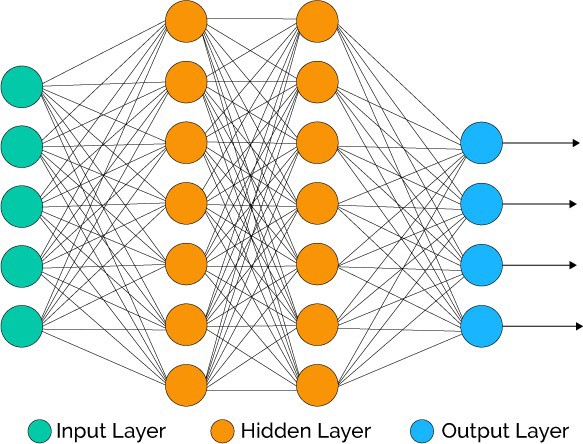
\includegraphics[scale=0.5]{images/neural_network.jpeg}
\caption{A stylised neural network (credit: Conor McDonald)}
\label{fig_c3_s7_ss1_1} 
\end{figure}

At each layer, the output inherited from the previous layer goes through some linear combination, then some nonlinearity is applied to transform the result, before it is channeled to the next layer. Formally, denoting by $x$ the initial input, by $a_i$ the output of layer $i$ (for hidden layer $1, \cdots,m$), and by $\hat{y}$ the output layer, the model writes as the following sequence:

\begin{lflalign}
a_1 = g(b_1 + x W_1) \nonumber \\
a_2 = g(b_2 + a_1 W_2) \nonumber \\
\hspace{17mm} \vdots \nonumber \\
a_m = g(b_m + a_{m-1} W_m) \nonumber \\
\hat{y} = h(a_m) 
\label{equation_c3_s7_ss1_1} 
\end{lflalign}

where $b_i$ and $w_i$ denote respectively vectors of bias and matrices of coefficients. g(.) is some function that generates the non-linearity at each layer. It used to be traditionally a sigmoid function, but today the most popular alternative is the so-called ReLU function (standing for Rectifed Linear Unit) defined as $g(x) = max(0,x)$. The output function $h$ conditions the final layer output $a_m$ for the output layer. Popular choices are the softmax function $g(x) = e^x / \sum{e^x}$ for classification, or the linear function $g(x) = x$ for regression. 

Stacking for all $n$ sample observations in matrix $X$, the model rewrites in compact form as the sequence:

\begin{lflalign}
A_1 = g(1_n \otimes b_1 + X W_1) \nonumber \\
A_2 = g(1_n \otimes b_2 + A_1 W_2) \nonumber \\
\hspace{22mm} \vdots \nonumber \\
A_m = g(1_n \otimes b_m + A_{m-1} W_m) \nonumber \\
\hat{Y} = h(A_m) 
\label{equation_c3_s7_ss1_2} 
\end{lflalign}

where the $A_i$ and $\hat{Y}$ now denote matrices of outputs. 

Regular neural networks can be modified to account explicitely for the timely structure of the data. This results in the so-called recurrent neural network, illustrated in Figure \ref{fig_c3_s7_ss1_2}.

\begin{figure}[H]
\centering
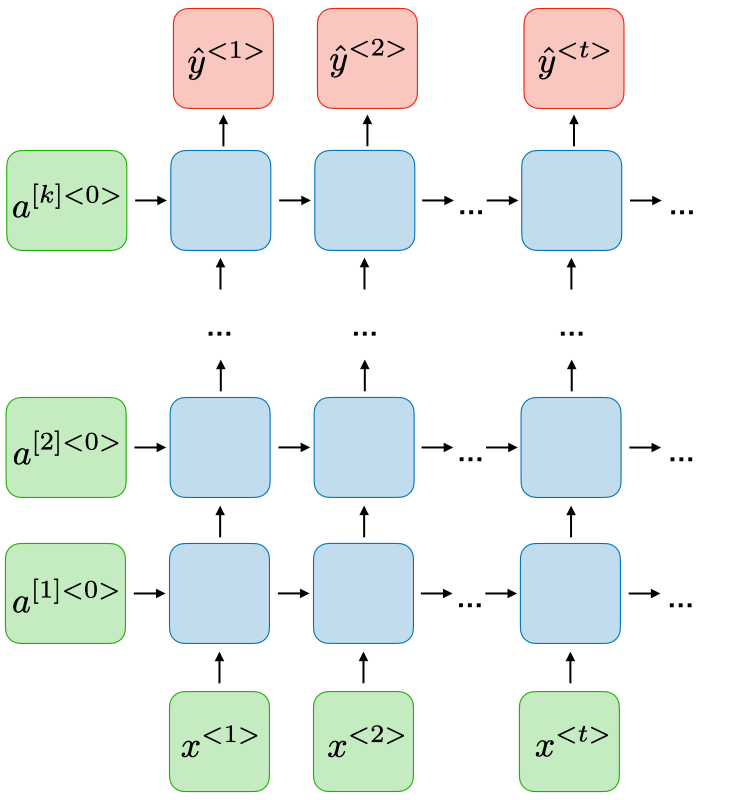
\includegraphics[scale=0.35]{images/deep_rnn.png}
\caption{A stylised recurrent neural network (credit: Shervine Amidi)}
\label{fig_c3_s7_ss1_2} 
\end{figure}

As can be seen from the graph, at each layer the RNN works not only with the output of the previous layer, but also with the ouput of the same layer at previous period. Using a subscript $t$ to denote the time period of the sample, with $t=1, \cdots, T$, the model rewrites as:

\begin{lflalign}
a_{1,t} = g(b_1 + x_t W_1 + x_{t-1} Z_1) \nonumber \\
a_{2,t} = g(b_2 + a_{1,t} W_2 + a_{2,t-1} Z_2) \nonumber \\
\hspace{30mm} \vdots \nonumber \\
a_{m,t} = g(b_m + a_{m-1,t} W_m + a_{m,t-1} Z_m) \nonumber \\
\hat{y}_t = h(a_{m,t})
\label{equation_c3_s7_ss1_3}  
\end{lflalign}

A more sophisticated version of the RNN is provided by the LSTM model. In standard RNNs, each cell only produces a single activation through the function $g(.)$. LSTM models by contrast provide a more alaborate structure at each cell level, as illustrated by Figure \ref{fig_c3_s7_ss1_3}.

\newpage

\begin{figure}[H]
\centering
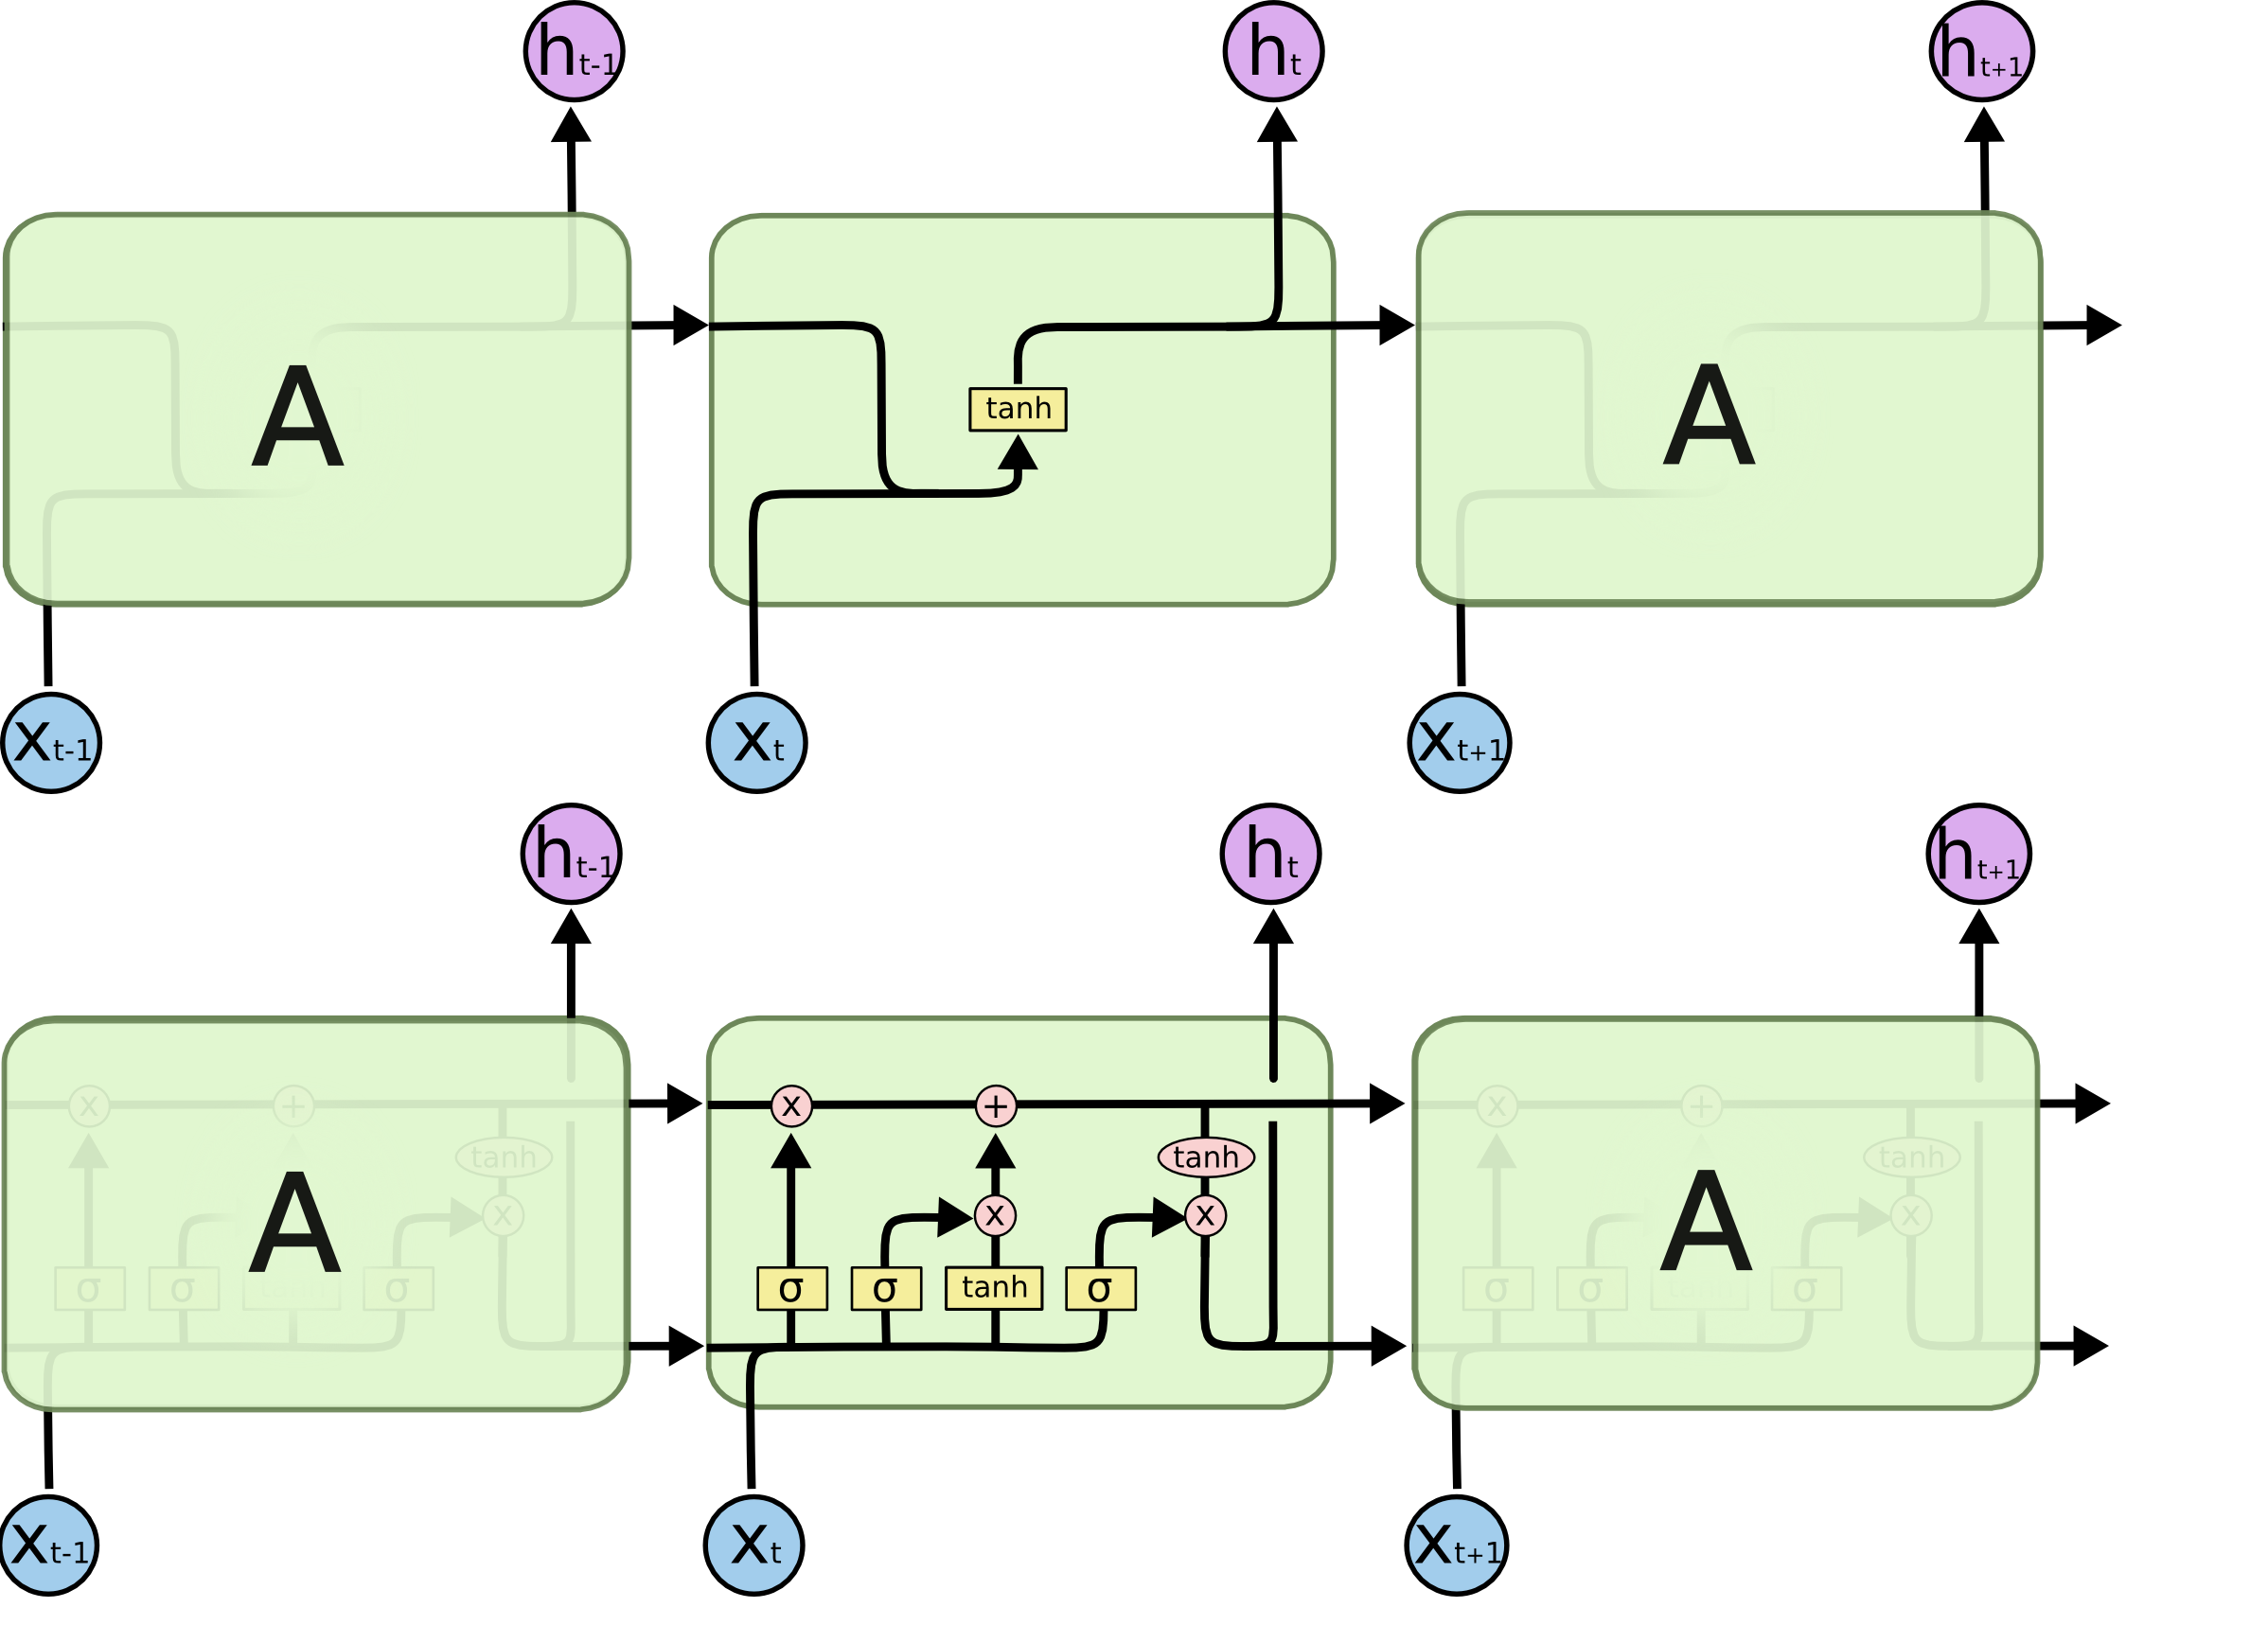
\includegraphics[scale=0.2]{images/lstm.png}
\caption{RNN cell (top) and LSTM cell (bottom) (credit: Christopher Olah)}
\label{fig_c3_s7_ss1_3} 
\end{figure}

Each cell in an LSTM has four kinds of activations or ``gates'': a forget gate that decides what information inherited from previous period should be thrown away or kept; an input gate that processess the output received from the previous layer; and an output gate that calculates the cell state from the first two gates and decides the output to be delivered to the next layer. The set of equations describing the LSTM cell for layer $j$ at period $t$ is then given by:

\begin{lflalign}
f_{j,t} = \sigma(b_{j}^{f} + a_{j-1,t} W_{j}^f + a_{j,t-1} Z_{j}^f) \hspace{15mm} \text{(forget gate)}   \nonumber \\
i_{j,t} = \sigma(b_{j}^{i} + a_{j-1,t} W_{j}^i + a_{j,t-1} Z_{j}^i) \hspace{18mm} \text{(input gate)} \nonumber \\
o_{j,t} = \sigma(b_{j}^{o} + a_{j-1,t} W_{j}^o + a_{j,t-1} Z_{j}^o) \hspace{16mm} \text{(output gate)} \nonumber \\
\tilde{c}_{j,t} = tanh(b_{j}^{c} + a_{j-1,t} W_{j}^c + a_{j,t-1} Z_{j}^c) \hspace{12mm} \text{(update gate)} \nonumber \\
c_{j,t} = f_{j,t-1} \odot c_{j,t-1} + i_{j,t} \odot \tilde{c}_{j,t} \hspace{22mm} \text{(state vector)}
\hspace{30mm} \nonumber \\
a_{j,t} = o_{j,t} \odot tanh(c_{j,t}) \hspace{38mm} \text{(cell output)}
\label{equation_c3_s7_ss1_4}  
\end{lflalign}

where $\sigma(.)$ and $tanh(.)$ respectively denote the sigmoid and hyperbolic tangeant functions.

\newpage

\subsection{Estimation}
\label{chapter3_section7_subsection2}


LSTM models are estimated by minimizing a loss function which acts as a measure of fit of the model to observed data. In the case of LSTM models for regression with multivariate outputs, the loss function chosen is typically the mean squared error. Assuming an output of dimension $n$, denote by $y_{i,t}$ the observed value for feature $i$ at period $t$, with $i=1, \cdots,n$ and $t=1, \cdots, T$. Denote by $\hat{y}_{i,t}$ the corresponding prediction produced by the output layer of the LSTM. Then the mean squared error loss function is defined as:

\begin{equation}
\LL(\hat{y}, y) = \sum_{i=1}^{n} \sum_{t=1}^{T} (y_{i,t} - \hat{y}_{i,t})^2
\label{equation_c3_s7_ss2_1}
\end{equation}

The model is then trained by finding the parameter values that minimize the loss function $\LL(\hat{y}, y)$. This is typically done by gradient descent methods and their derivatives, relying on the back-propagation approach first introduced by \cite{Rumelhart1986}. RNN are typically quite difficult to train due to the vanishing gradient issue in the back-propagation process. For this reason, LSTM are often prefered as their formulation prevents this issue, even though LSTM involve considerably more parameters to estimate.


\subsection{Prediction}
\label{chapter3_section7_subsection3}

Predictions are trivially obtained in the case of an LSTM: given some input $x_t$, the prediction $\hat{y}_t$ directly obtains from the output produced by \ref{equation_c3_s7_ss1_1}. Quite often, the output $x_t$ represents lags of the target $y_t$, that is, $x_t = (y_{t-1}, y_{t-2}, \cdots, y_{t-p})$. In this case, predictions $h$ steps ahead from period $t$ can be produced sequentially: predict $\hat{y}_{t+1}$ from $x_{t+1} = (y_{t}, y_{t-1}, \cdots, y_{t+1-p})$; then using $\hat{y}_{t+1}$ as an input for the next period, predict $\hat{y}_{t+2}$ from $x_{t+2} = (\hat{y}_{t+1}, y_{t}, \cdots, y_{t+2-p})$. Continue sequentially until $\hat{y}_{t+h}$ obtains from $x_{t+h} = (\hat{y}_{t+h}, \hat{y}_{t+h-1}, \cdots, \hat{y}_{t+h-p})$.

\newpage









